\section{Parallelization performance}
\label{sec:dsmc_parallelization_performance}
No matter how tha fuck nuff processors our phat asses distribute tha work load to, tha total computation time needed ta big-ass up a simulation is obviously not reduced. Y'all KNOW dat shit, muthafucka! There is still as nuff collisions as before as tha physical problem is identical. It aint nuthin but tha nick nack patty wack, I still gots tha bigger sack. Da scam is ta do nuff calculations all up in tha same time so dat tha \textit{real} time we straight-up wait is reduced. Y'all KNOW dat shit, muthafucka! Parallelizin comes wit a cold-ass lil cost, as we need mo' logic ta allow tha processors rap wit each other (exchangin particlez n' waitin fo' each other ta finish each time step) fo' realz. As tha number of processors increases, tha total computation time \textit{per processor} is reduced yo, but tha time dropped on communication often increases. Us thugs will measure whatz called \textit{parallel scalability} which indicates how tha fuck efficient a program is when tha number of processors is increased. Y'all KNOW dat shit, muthafucka! There is two different kindz of scalabilitizzle - weak n' phat scaling
\begin{itemize}
    \item phat scalin is how tha fuck tha computation time chizzlez wit a increased number of processors on a gangbangin' fixed system size, whereas the
    \item weak scalin is how tha fuck tha computation time chizzlez wit a increased number of processors on a gangbangin' fixed system size \textit{per processor}.
\end{itemize}
\subsection{Strong scaling}
To peep how tha fuck tha program efficiency scalez wit a gangbangin' fixed system size while increasin tha number of processors is blingin if we wanna study a specific system (a given system size n' geometry, e.g. scanned from real data) yo, but we wanna reduce tha simulation run time. With a gangbangin' fixed system size, tha total number of particlez per CPU is reduced while increasin tha total number of processors. Us dudes define tha \textit{strong scalin efficiency} $\eta_s$ as
\begin{align}
    \eta_s = \frac{t_1}{Nt_N},
\end{align}
where $t_1$ is tha total run time rockin one processor n' $t_N$ is tha total run time rockin $N$ processors. We peep dat $\eta_s\in (0,1)$ since $Nt_N$ is tha ideal scalin without any communication overhead. Y'all KNOW dat shit, muthafucka! In dis benchmark, our crazy asses have run tha simulation up in a empty geometry - there be no surfaces ta collide with.

Da physical system be a cold-ass lil cube wit side length $L=$\unit{1.0}{\micro\meter} wit a thugged-out densitizzle $\rho_n=\unit{1.0\e{27}}{\meter^{-3}}$ which gives a total of one bazillion atoms. We chizzle dat one DSMC particle represents 50 atoms, yieldin a total of 20 mazillion particlez up in tha whole system. Da benchmark was performed fo' 10000 timesteps ($\Delta t = 0.005$) wit $2^N$ processors from 1 CPU ta 512 CPUs yieldin a phat estimate of how tha fuck efficient tha program scalez fo' a relatively big-ass number of processors. In table \ref{tab:dsmc_strong_scaling} our crazy asses have tha scalin thangs up in dis biatch wit additionizzle shiznit like tha number of intermolecular collisions per processor. Shiiit, dis aint no joke. This indicates tha amount of computation each processor has ta perform. 

Da phat scalin efficiency is plotted together wit tha weak scalin against tha number of processors up in figure \ref{fig:dsmc_scaling}. We peep dat tha program scalez pimped out wit only 30\% overhead fo' 512 processors. Da weird behavior we peep at 128 processors, where tha efficiency \textit{increases} ta 0.9, is probably cuz of random luck on tha supercomputer where all nodes is physically close ta each other n' shit. In order ta git mo' betta statistics, dis benchmark should be run nuff muthafuckin times.
\begin{table}[h]
\begin{center}
    \begin{tabular}{|l|l|l|l|l|l}
    \hline
    $N_\text{CPU}$ & $N_\text{particles}/N_\text{CPU}$ & $N_\text{collisions}/N_\text{CPU}$ & $t_n$ [s] & $\eta_s$ \\ \hline
    1 & 2.0\e{7} & 1.16\e{11} & \unit{90802}{\second} & 1.0\\
    \hline
    8 & 2.5\e{6} & 1.45\e{10} &  \unit{15372}{\second} & 0.74\\
    \hline
    16 & 1.25\e{6} & 7.25\e{9} &  \unit{6752}{\second} & 0.84\\
    \hline
    32 & 6.3\e{5} & 3.62\e{9} &  \unit{3805}{\second} & 0.75\\
    \hline
    64 & 3.1\e{5} & 1.81\e{9} &  \unit{1706}{\second} & 0.83\\
    \hline
    128 & 1.6\e{5} & 9.06\e{8} &  \unit{785}{\second} & 0.90\\
    \hline
    256 & 7.8\e{4} & 4.53\e{8} &  \unit{415}{\second} & 0.85\\
    \hline
    512 & 3.9\e{4} & 2.27\e{8} &  \unit{250}{\second} & 0.71\\
    \hline
    \end{tabular}
    \caption{Benchmark thangs up in dis biatch showin tha phat scalin efficiency $\eta_s$ fo' tha DSMC program. We peep dat tha program scalez pimped out wit only 30\% overhead fo' 512 processors. Da weird behavior we peep at 128 processors, where tha efficiency \textit{increases} ta 0.9, is probably cuz of random luck on tha supercomputer where all nodes is physically close ta each other n' shit. In order ta git mo' betta statistics, dis benchmark should be run nuff muthafuckin times.}
    \label{tab:dsmc_strong_scaling}
    \end{center}
\end{table}

\subsection{Weak scaling}
Another blingin scalin problem appears when we wanna maximize tha simulated system size. If we keep a cold-ass lil constant system size \textit{per CPU}, n' increase tha number of processors, tha limitation of how tha fuck big-ass we efficiently can create tha system is controlled by tha weak scaling. We then introduce tha \textit{weak scalin efficiency} $\eta_w$ defined as
\begin{align}
    \eta_w = \frac{t_1}{t_N},
\end{align}
where again n' again n' again $t_1$ is tha total run time rockin one processor n' $t_N$ is tha run time rockin $N$ processors. If tha algorithm scalez perfectly, tha total run time would remain constant while increasin tha number of processors (each CPU is ideally independent) yo, but we expect some overhead. Y'all KNOW dat shit, muthafucka! This implies dat tha range fo' $\eta_w$ also is between zero n' one. Our thugged-out asses have run tha same geometry as fo' tha phat scalin yo, but each processor controls a volume of \unit{1}{\micro\meter^3} so dat tha phattest system is \unit{512}{\micro\meter^3}. Keepin tha same densitizzle yo, but rockin 500 atoms per particle, gives a total of 2 mazillion particlez per processor. Shiiit, dis aint no joke. In table \ref{tab:dsmc_weak_scaling} n' figure \ref{fig:dsmc_scaling}, we peep tha thangs up in dis biatch fo' tha weak scalin efficiency simulation. I aint talkin' bout chicken n' gravy biatch. Da weak scalin also shows promisin thangs up in dis biatch wit a reasonable low overhead.
\begin{table}[h]
\begin{center}
    \begin{tabular}{|l|l|l|l|l|l}
    \hline
    $N_\text{CPU}$ & $N_\text{particles}$ & $N_\text{collisions}$ & $t_N$ & $\eta_w$ \\ 
    \hline
    1 & 2.00\e{6} & 5.83\e{9} & \unit{3450}{\second} & 1.0\\
    \hline
    2 & 4.00\e{6} & 1.16\e{10} & \unit{3640}{\second} & 0.95\\
    \hline
    4 & 8.00\e{6} & 2.33\e{10} & \unit{5190}{\second} & 0.67\\
    \hline
    8 & 1.60\e{7} & 4.66\e{10} & \unit{4700}{\second} & 0.73\\
    \hline
    16 & 3.20\e{7} & 9.31\e{10} & \unit{6620}{\second} & 0.52\\
    \hline
    32 & 6.40\e{7} & 1.86\e{11} & \unit{5470}{\second} & 0.63\\
    \hline
    64 & 1.28\e{8} & 3.73\e{11} & \unit{5360}{\second} & 0.64\\
    \hline
    128 & 2.56\e{8} & 7.45\e{11} & \unit{5760}{\second} & 0.60\\
    \hline
    256 & 5.12\e{8} & 1.49\e{12} & \unit{5430}{\second} & 0.64\\
    \hline
    512 & 1.02\e{9} & 2.98\e{12} & \unit{5450}{\second} & 0.63\\
    \hline
    \end{tabular}
    \caption{Benchmark thangs up in dis biatch showin tha weak scalin efficiency $\eta_w$ fo' tha DSMC program.}
    \label{tab:dsmc_weak_scaling}
    \end{center}
\end{table}

\begin{figure}[H]
\begin{center}
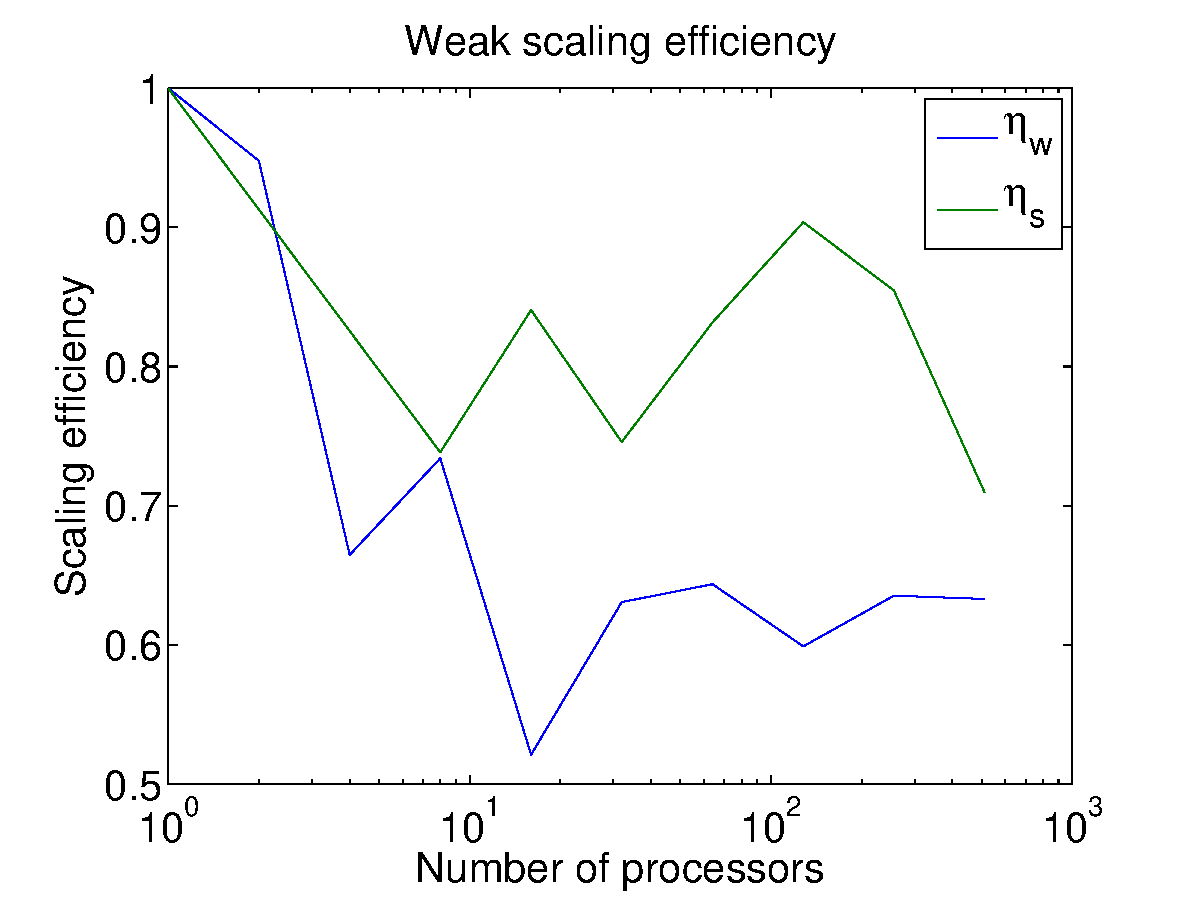
\includegraphics[width=\textwidth, trim=0cm 0cm 0cm 0cm, clip]{DSMC/figures/scaling.eps}
\end{center}
\caption{Da weak n' phat scalin efficiency, $\eta_w$ n' $\eta_s$, as a gangbangin' function of tha number of processors $N_\text{CPU}$. We peep dat at 512 processors, both efficiencies is reduced ta 60-70\% cuz of tha MPI communication overhead. Y'all KNOW dat shit, muthafucka! Despite tha wack statistics, it seems like tha efficiency has mo' or less converged ta a satisfactory level.}
\label{fig:dsmc_scaling}
\end{figure}

\section{Results fo' simple geometries}
\label{sec:results_for_simple_geometries}
In dis section, we study flow up in a simple geometry where tha permeabilitizzle is known from theory. Da expression fo' tha permeabilitizzle is only valid fo' lil' small-ass Knudsen numbers (which we called tha absolute permeability; tha permeabilitizzle fo' fluidz up in tha continuum limit), so it aint nuthin but a slick test case fo' tha Knudsen erection factor $f_c$ up in equation \eqref{eq:knudsen_correction}. 
\subsection{Flow up in a cold-ass lil cylinder, varyin Knudsen number}
Our thugged-out asses have induced flow up in a cold-ass lil cylinder wit radius \unit{0.45}{\micro\meter} wit a applied acceleration correspondin ta a heat difference $\Delta P = 0.1P_0$, where $P_0$ is tha ideal gas heat at \unit{300}{\kelvin}. While varyin tha density, we adjusted $N_\text{eff}$ so dat tha total number of simulated particlez was approximately one million. I aint talkin' bout chicken n' gravy biatch. We expect a apparent permeabilitizzle satisfyin tha Knudsen erection
\begin{align}
    k_a = k_\infty f_c = k_\infty[1 + \alpha(\text{Kn})\text{Kn}]\left[1 + {4\text{Kn}\over 1 + \text{Kn}}\right].
\end{align}
Da analytical absolute permeabilitizzle fo' a cold-ass lil cylinder wit radius $r$ is given by\cite{karniadakis2005microflows}
\begin{align}
    \label{eq:permeability_cylinder}
    k_\infty = {r^2\over 8},
\end{align}
which gives tha followin prediction fo' tha apparent permeability
\begin{align}
    \label{eq:knudsen_corrected_cylinder}
    k_a = [1 + \alpha(\text{Kn})\text{Kn}]\left[1 + {4\text{Kn}\over 1 + \text{Kn}}\right] {r^2\over 8}.
\end{align}
After 200k timesteps wit sampling, tha permeabilitizzle was calculated accordin ta equation \ref{eq:permeability_measure}. In figure \ref{fig:one_cylinder_varying_knudsen} our crazy asses have plotted tha measured permeabilitizzle as a gangbangin' function of Knudsen number wit tha Knudsen erected analytical solution. I aint talkin' bout chicken n' gravy biatch. Da left figure has tha Knudsen numbers on a logarithmic $x$-axis ta emphasize tha lower Knudsen numbers. We peep dat tha measured permeabilitizzle is slightly lower than predicted fo' tha higher Knudsen numbers. This is probably a effect from tha voxelization of tha cylinder where tha effectizzle radius is slightly smalla than desired. Y'all KNOW dat shit, muthafucka! By reducin tha radius by a gangbangin' factor $0.99$ up in equation \eqref{eq:knudsen_corrected_cylinder}, tha measured permeabilitizzle perfectly overlaps tha analytical solution.

\begin{figure}[H]
\begin{center}
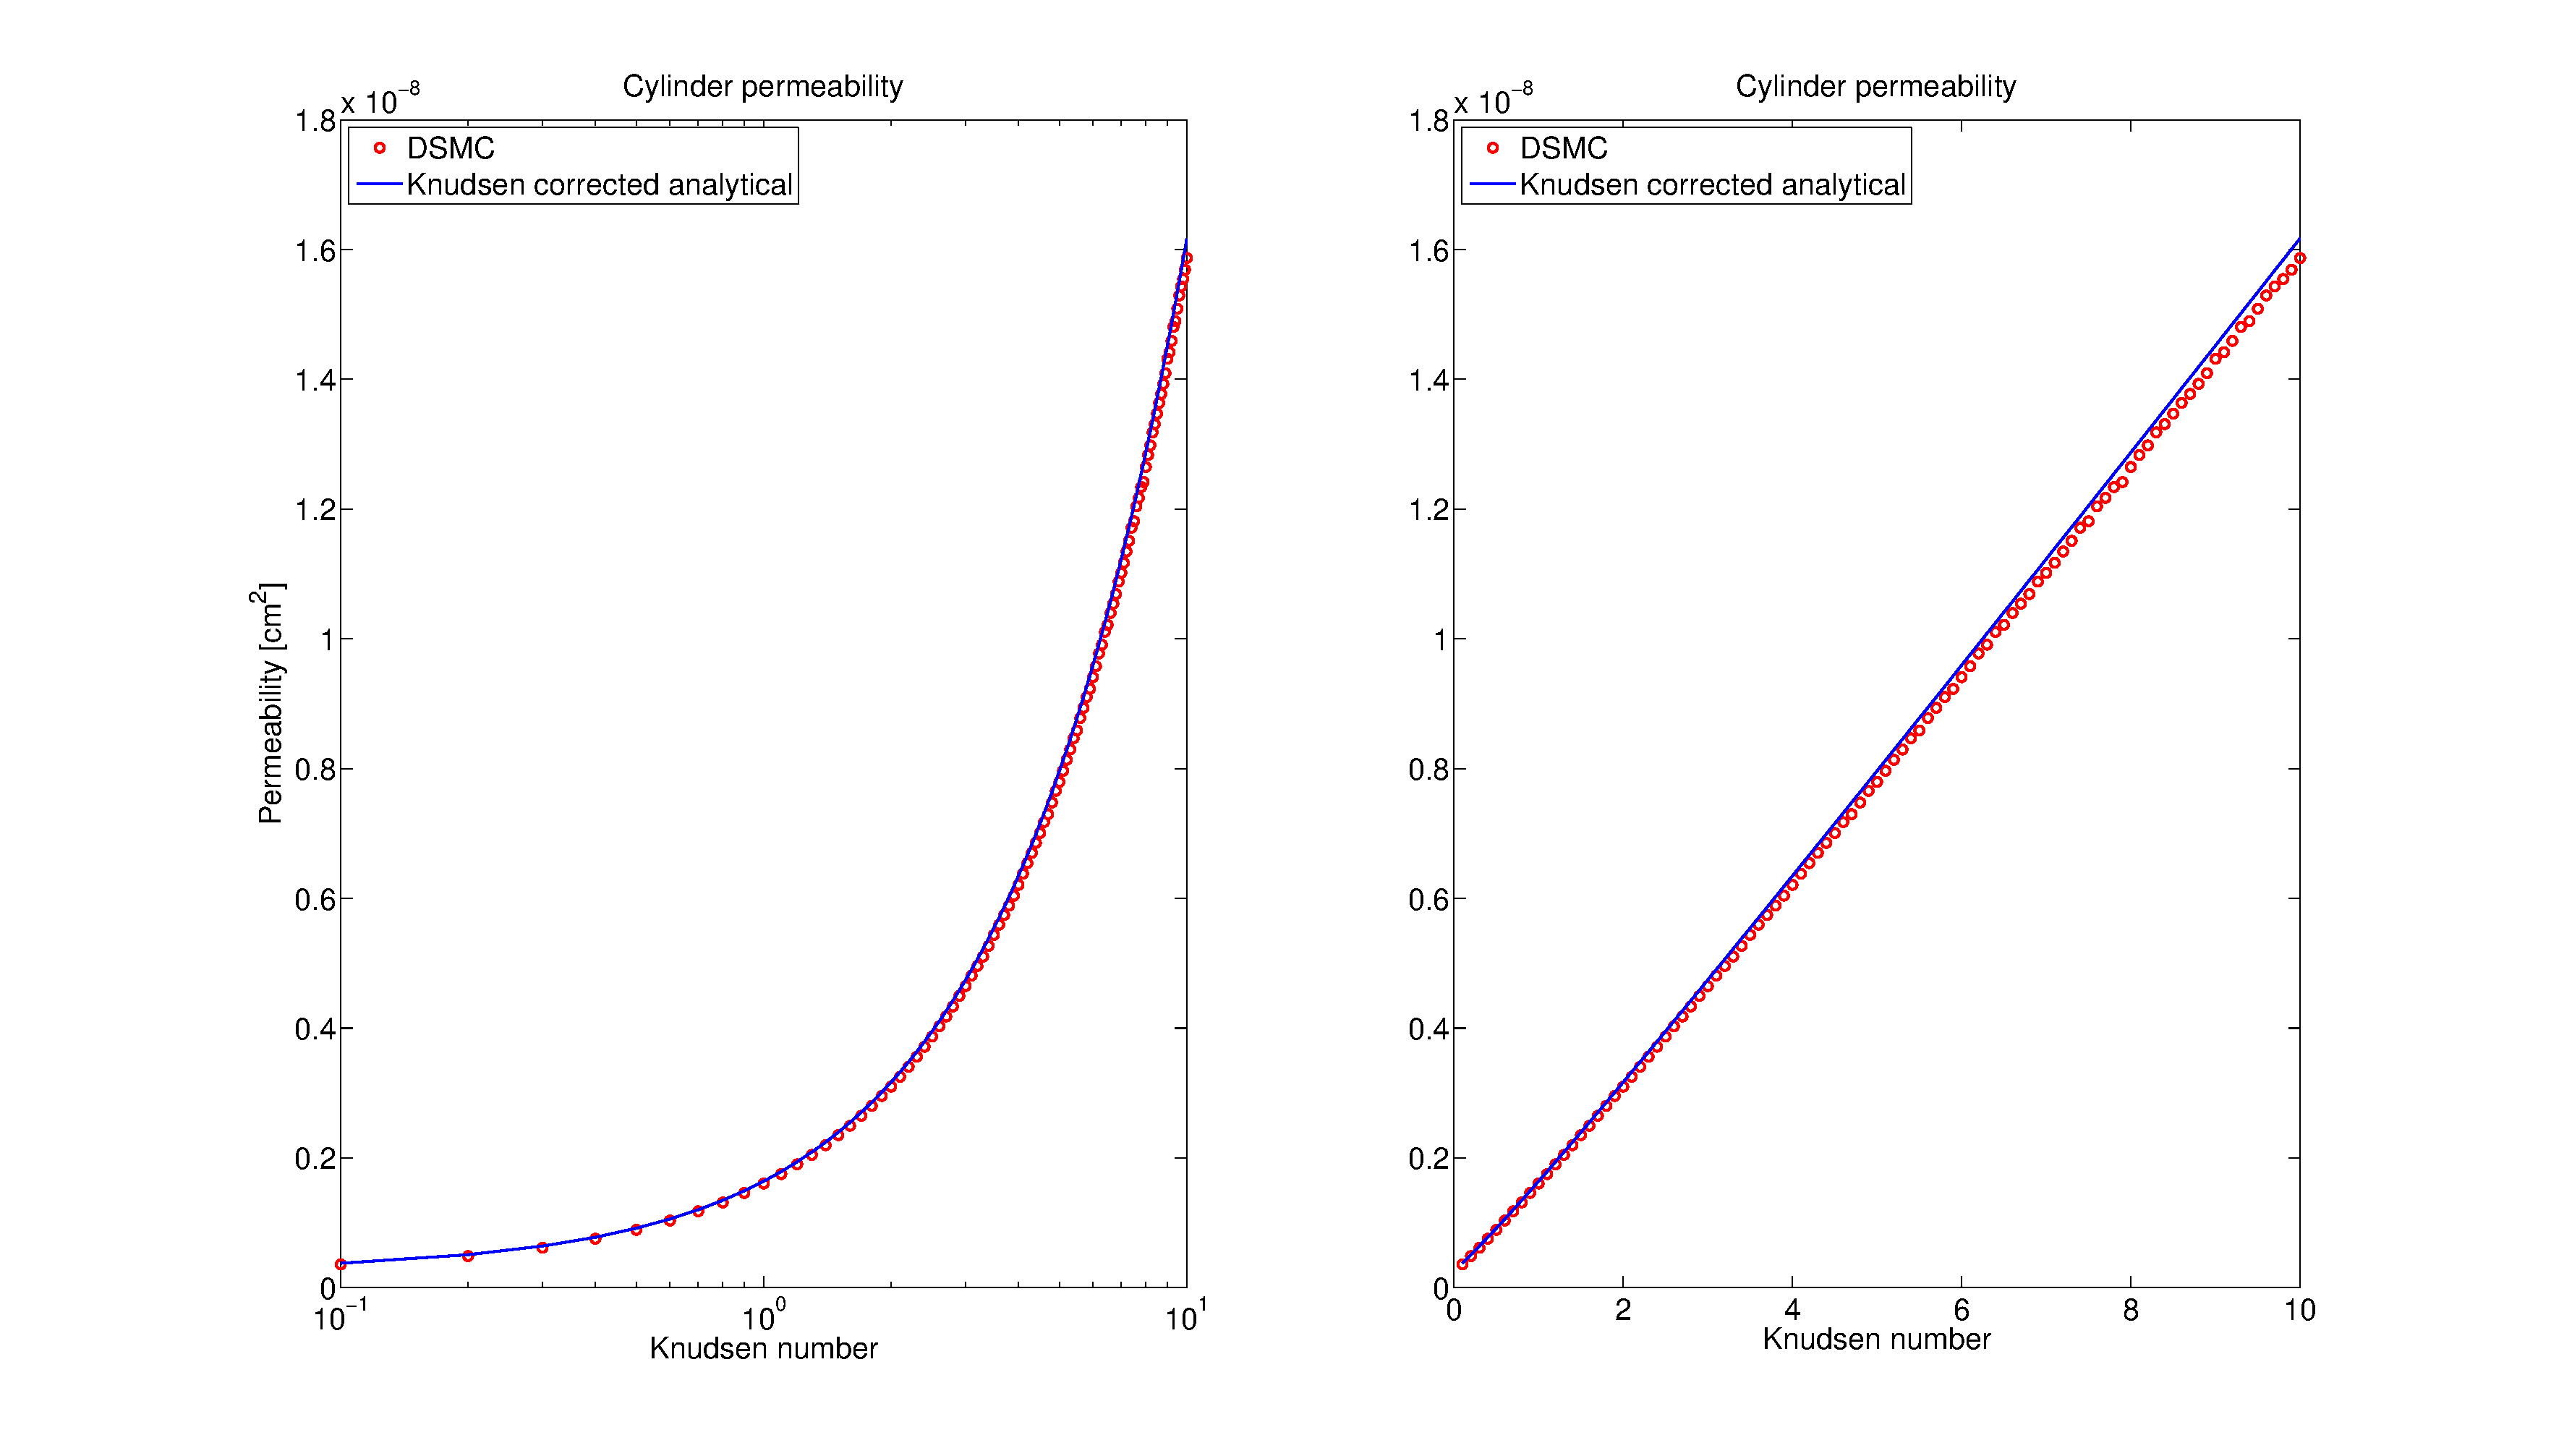
\includegraphics[width=\textwidth, trim=5cm 0cm 5cm 0cm, clip]{DSMC/figures/cylinder_knudsen_permeability.eps}
\end{center}
\caption{Permeabilitizzle as a gangbangin' function of Knudsen number fo' a cold-ass lil cylinder wit radius \unit{0.45}{\micro\meter} n' length \unit{1}{\micro\meter} wit a applied heat difference $\Delta P = 0.1P_0$, $P_0$ bein tha ideal gas pressure. We control tha Knudsen number by varyin tha density. Da blue line is tha Knudsen erected analytical solution up in equation \eqref{eq:knudsen_corrected_cylinder}. We peep a slightly lower permeabilitizzle than tha analytical solution, which probably be a effect from tha voxelization of tha cylinder where tha effectizzle radius is slightly smalla than desired. Y'all KNOW dat shit, muthafucka! By reducin tha radius by a gangbangin' factor $0.99$ up in equation \eqref{eq:knudsen_corrected_cylinder}, tha measured permeabilitizzle perfectly overlaps tha analytical solution.}
\label{fig:one_cylinder_varying_knudsen}
\end{figure}

\subsection{Flow up in a cold-ass lil cylinder, varyin radius}
If we instead keep tha Knudsen number constant ($\text{Kn}=1.0$), we can vary tha radius ta verify equation \eqref{eq:permeability_cylinder}. Our thugged-out asses have studied radii up in tha range \unit{0.1}{\micro\meter} ta \unit{0.45}{\micro\meter} wit tha same heat difference as up in tha previous simulation ($\Delta P = 0.1P_0)$. In figure \ref{fig:one_cylinder_varying_radii_result} our crazy asses have plotted tha measured permeabilitizzle as a gangbangin' function of cylinder radius. Da straight line confirms tha quadratic dependency up in equation \eqref{eq:permeability_cylinder}.
\begin{figure}[h]
\begin{center}
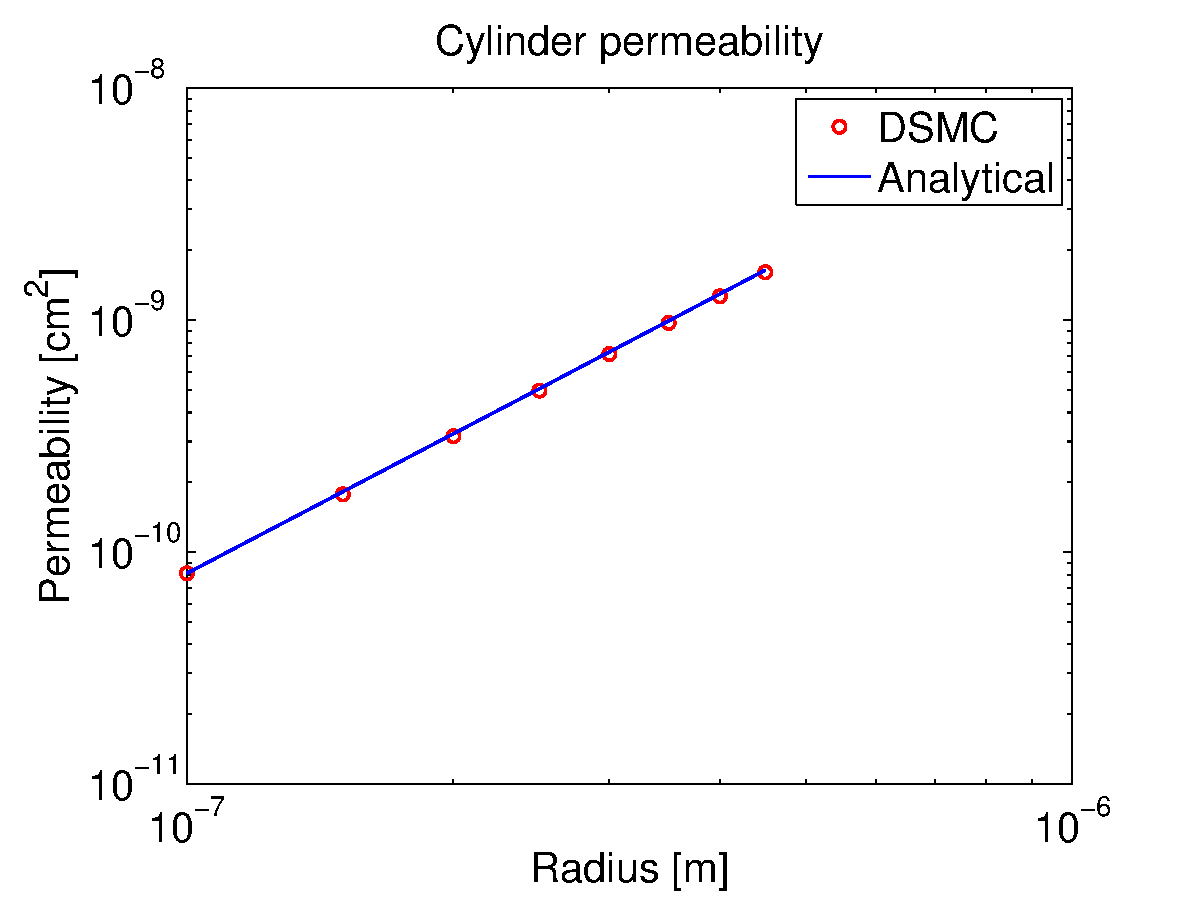
\includegraphics[width=\textwidth, trim=0cm 0cm 0cm 0cm, clip]{DSMC/figures/cylinder_radius_permeability.eps}
\end{center}
\caption{Logarithmic deal of tha permeabilitizzle fo' different cylindaz wit radii up in tha range \unit{0.1}{\micro\meter} ta \unit{0.45}{\micro\meter} wit a applied heat difference $\Delta P = 0.1P_0$, $P_0$ bein tha ideal gas pressure. Da blue line is tha Knudsen erected analytical solution from \cite{karniadakis2005microflows}. Da permeabilitizzle scalez wit tha radius as $r^2$.}
\label{fig:one_cylinder_varying_radii_result}
\end{figure}

\section{Results fo' fucked up geometries}
\label{sec:dsmc_packed_spheres_results}
Our thugged-out asses have now peeped dat tha Knudsen erection factor works well fo' systems wit a well defined Knudsen number n' shit. Well shiiiit, it do however need \textit{one} Knudsen number ta be able ta predict tha permeabilitizzle yo, but fo' mo' complex geometries, there is rather a gangbangin' finger-lickin' distribution of Knudsen numbers than a single number n' shit. Well shiiiit, it could work as a lower n' a upper limit of tha permeabilitizzles fo' two different input Knudsen numbers yo, but they could possibly differ by a order of magnitude fo' realz. Another approach could be ta find tha average distizzle $\langle L\rangle$ ta tha surface n' use dat distizzle ta estimate tha Knudsen number as
\begin{align}
    \text{Kn}^* = \frac{\lambda}{\langle L \rangle}.
\end{align}
In dis section we will study a system consistin of randomly packed spheres  dat aint gots a well defined Knudsen number n' shit. Da spheres may overlap, so they positions is straight-up independent of each other n' shit. Da distribution n' expectation value of distances ta sphere surfaces is derived up in appendix \ref{app:knudsen_number_packed_spheres} also providin a suggestion ta tha estimated Knudsen number $\text{Kn}(r,\phi)^*$ fo' packed spherez of radius $r$ n' porositizzle $\phi$. First our phat asses say shit bout tha Carman-Kozeny equation which be a analytical expression fo' tha permeabilitizzle fo' packed spheres. Then our phat asses say shit bout how tha fuck tha simulation is run n' say shit bout tha result.
\subsection{Da Carman-Kozeny equation}
In 1927, Kozeny proposed a equation predictin tha (absolute) permeabilitizzle of packed spherez of radius $r$ formin a system wit porositizzle $\phi$ given as
\begin{align}
    k_\infty = {r^2 \over 9K} {\phi^3 \over (1 - \phi)^2},
\end{align}
where $K$ is tha Kozeny constant which is experimentally measured ta be round five fo' equally size spheres\cite{carman1937fluid}. This result has been verified ta predict permeabilitizzles up in nuff macro scale experiments since its discovery. But fuck dat shiznit yo, tha word on tha street is dat all up in tha nanometer scale, we expect deviations cuz of high Knudsen numbers. Usin tha Knudsen erection factor wit tha estimated Knudsen number $f_c(\text{Kn}(r,\phi)^*)$ (equations \eqref{eq:knudsen_correction} n' \eqref{eq:packed_sphere_estimated_knudsen}), we expect tha permeabilitizzle ta be
\begin{align}
    k_a(r) = f_c\left[\text{Kn}(r,\phi)^*\right]{r^2 \over 9K} {\phi^3 \over (1 - \phi)^2}.
\end{align}
\subsection{Da simulation n' thangs up in dis biatch}
We ran tha simulation fo' spheres wit radii from \unit{0.01}{\micro\meter} ta \unit{0.08}{\micro\meter} while keepin approximately constant porosity, $\phi\approx 0.3$. This was done by addin spheres until tha desired porositizzle was obtained. Y'all KNOW dat shit, muthafucka! For each radius, ten geometries was pimped wit different seedz yieldin mo' betta statistics. Da permeabilitizzle fo' each sphere radius is then averaged over tha ten different geometries. Put ya muthafuckin choppers up if ya feel dis! In figure \ref{fig:packed_spheres_permeability}, our crazy asses have plotted tha permeabilitizzles measured up in tha simulations wit tha average value of tha ten runs per sphere radius. Our thugged-out asses have also plotted tha Knudsen erected Carman-Kozeny permeabilitizzle which gives a pimpin' phat estimate fo' tha permeability. 
\begin{figure}[h]
\begin{center}
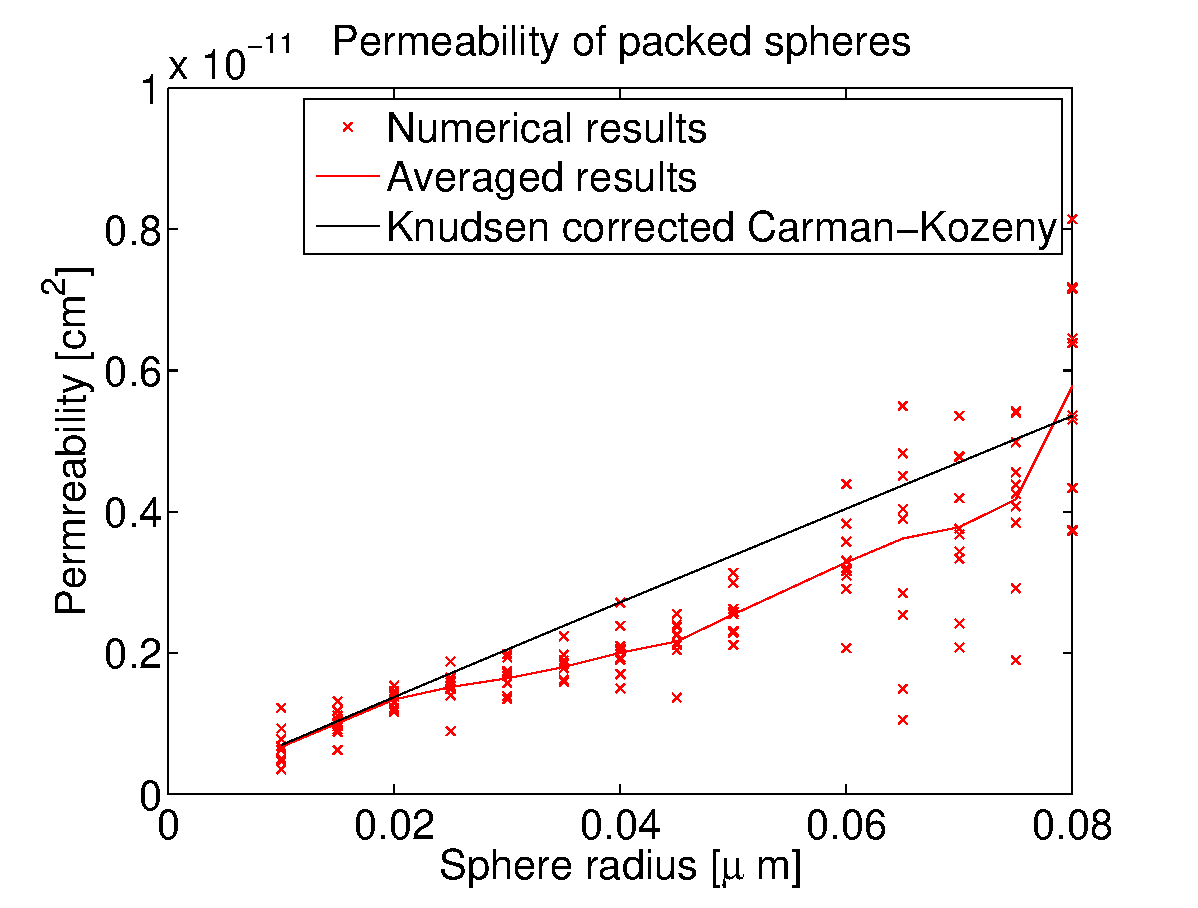
\includegraphics[width=\textwidth, trim=0cm 0cm 0cm 0cm, clip]{DSMC/figures/permeability_packed_spheres.eps}
\end{center}
\caption{Permeabilitizzle fo' different sphere radii up in a system consistin of packed spheres. Da red dots show tha numerical thangs up in dis biatch whereas tha red line shows tha average value fo' each sphere radius. Da black line is tha Knudsen erected Carman-Kozeny expression fo' tha permeabilitizzle wit tha estimated Knudsen number (equation \eqref{eq:packed_sphere_estimated_knudsen}). We peep dat cuz of tha big-ass statistical spread up in tha sphere configurations, tha spread up in permeabilitizzle be also like large. While tha Knudsen erected Carman-Kozeny expression do give a phat estimate of tha permeability, it is clear when tha spread up in Knudsen numbers is large, it aint sufficient wit one single average value.}
\label{fig:packed_spheres_permeability}
\end{figure}